\documentclass{article}

\usepackage{fontspec}
\setmainfont{Libertinus Serif}
\usepackage[margin=1in]{geometry}
\usepackage{tikz}
\usetikzlibrary{arrows.meta}
\usetikzlibrary{positioning}
\usetikzlibrary{quotes}

\setlength{\parindent}{0pt}

\newcommand{\chapelmaster}[3]{%
    \begin{tabular}{c}
        #1\\
        #2\\[1ex]
        #3
    \end{tabular}%
}
\newcommand{\Puebla}{\textsc{Puebla Cathedral}}
\newcommand{\Fernandez}{%
    \chapelmaster
    {Gaspar Fernández}
    {(15xx--1628)}
    {MC 16xx--1628}%
}
\newcommand{\Padilla}{%
    \chapelmaster
    {Juan Gutiérrez de Padilla}
    {(1590--1664)}
    {MC 1628--1664}%
}
\newcommand{\Garcia}{%
    \chapelmaster
    {Juan García de Céspedes}
    {(16xx--16xx)}
    {MC 16xx--16xx}%
}
\newcommand{\Sevilla}{\textsc{Seville Cathedral}}
\newcommand{\Lobo}{%
    \chapelmaster
    {Alonso Lobo}
    {(15xx--1616)}
    {MC 15xx--1616}%
}
\newcommand{\Santiago}{%
    \chapelmaster
    {Fray Francisco de Santiago}
    {(15xx--1644)}
    {MC 1617--1644}%
}
\newcommand{\Jalon}{%
    \chapelmaster
    {Luis Bernardo Jalón}
    {(16xx--16xx)}
    {MC 1644--16xx}%
}

% \newcommand{\Vidales}{Vidales}
% \newcommand{\Vasquez}{Vásquez}
% \newcommand{\Dupont}{Dupont}
\begin{document}
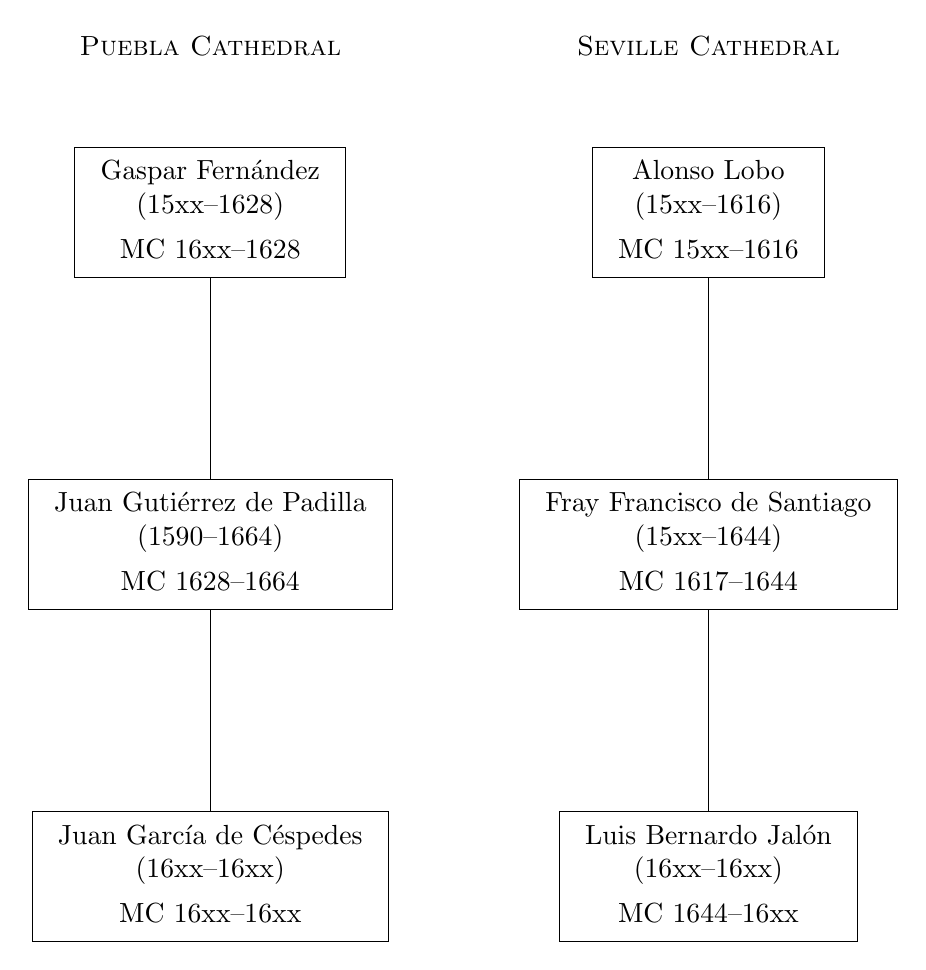
\begin{tikzpicture}[sibling distance=18em,
                    level 1/.style={
                        level distance=0pt,
                        edge from parent/.style={draw=none}
                    },
                    level 2/.style={
                        level distance=6em,
                        edge from parent/.style={draw=none},
                        every child node/.style={draw}
                    },
                    level 3/.style={
                        level distance=12em,
                        edge from parent/.style={draw},
                    }]

    \node (root) {}
        child { node (p0) {\Puebla}
            child { node (p1) {\Fernandez} 
                child { node (p2)  {\Padilla} 
                    child { node (p3) {\Garcia}
                    }
                }
            }
        }
        child { node (s0) {\Sevilla}
            child { node (s1) {\Lobo}
                child { node (s2) {\Santiago}
                    child { node (s3) {\Jalon}
                    }
                }
            }
        };
        
\end{tikzpicture}

\end{document}

